\documentclass[10pt,twocolumn,letterpaper]{article}

\usepackage{cvpr}
\usepackage{times}
\usepackage{epsfig}
\usepackage{amsmath}
\usepackage{amssymb}

\usepackage{booktabs} % for much better looking tables
\usepackage{array} % for better arrays (eg matrices) in maths
\usepackage{paralist} % very flexible & customisable lists (eg. enumerate/itemize, etc.)
\usepackage{verbatim} % adds environment for commenting out blocks of text & for better verbatim
\usepackage{subfigure} % make it possible to include more than one captioned figure/table in a single float
\usepackage{graphicx}
\usepackage{multirow}
% Include other packages here, before hyperref.

% If you comment hyperref and then uncomment it, you should delete
% egpaper.aux before re-running latex.  (Or just hit 'q' on the first latex
% run, let it finish, and you should be clear).
%\usepackage[pagebackref=true,breaklinks=true,letterpaper=true,colorlinks,bookmarks=false]{hyperref}

\cvprfinalcopy % *** Uncomment this line for the final submission

\def\cvprPaperID{****} % *** Enter the CVPR Paper ID here
\def\httilde{\mbox{\tt\raisebox{-.5ex}{\symbol{126}}}}

% Pages are numbered in submission mode, and unnumbered in camera-ready
\ifcvprfinal\pagestyle{empty}\fi
\begin{document}

%%%%%%%%% TITLE
\title{
Project in CSE 250B\\
Assignment 2: Logistic Regression with Regularization}

\author{Andreas Landstad, Spencer Bliven, Jonas Hoelzler\\
Computer Science Department\\
University of California, San Diego\\
{\tt\small landstad.andreas@gmail.com, sbliven@ucsd.edu, jonas@hoelzler.de}
}% For a paper whose authors are all at the same institution,
% omit the following lines up until the closing ``}''.
% Additional authors and addresses can be added with ``\and'',
% just like the second author.
% To save space, use either the email address or home page, not both
%\and
%Second Author\\
%Institution2\\
%First line of institution2 address\\
%{\tt\small secondauthor@i2.org}
\maketitle
\thispagestyle{empty}

%%%%%%%%% ABSTRACT
\begin{abstract}
This project evaluates an email analytics dataset describing two email campaigns and a control group using machine learning methods. The datasets is analyzed using logistic regression with stochastic gradient descent as optimization method and a real-valued nonlinear regression training method.
The results show that the outcome after applying the men�s email campaign is 0.77 USD higher than when no email advertisement was applied. For the women�s email campaign the outcome was 0.40 USD higher.
\end{abstract}

%%%%%%%%% BODY TEXT
\section{Description of the Dataset}
Kevin Hillstrom, a well-known data mining consultant has published an email analytics dataset with 64,000 records each describing a customer \cite{hillstrom08, radcliffe08}. One third of these customers were randomly chosen to receive an email referred to as the Men's email, a
second random third received a different email (the Women's email) and the remaining customers served as a control, receiving neither email.
The dataset is almost perfectly equally divided between the two mailings (�Men's� and �Women's�) and an untreated control group (see Table \ref{dataoverview}).


\begin{figure}[htbp]
    \centering

 \begin{tabular}{|l|l|l|l|l|}
  \hline
   Mailing & Men	& Women  & None   & Total   \\
   \hline
   Count & 21,307 & 21,387 & 21,306 & 64,000 \\
   \%   	& 33.29\% & 33.42\% & 33.29\% & 100.00\% \\
   
  \hline
 \end{tabular}

\caption{Partitioning of the email analytics dataset}
 \label{dataoverview}
\end{figure}

\section{Preprocessing: Feature Selection for Regression}
The data is given as a comma separated file. To apply the logistic and linear regressions, the data has to be preprocessed. For the learning algorithm, customer information is encoded as $x\in\mathbb{R}^{25}$. The encoding \ref{encoding} is described at the following.

First, the recency entry shows the number of months since the last purchase from one to twelve months. In this project it is encoded as a bit-vector of eleven bits (bit 1 to 11), where the $i$th bit is $'1'$ for a recency of $i$ months and $'0'$ otherwise. The $12$th bit is left out, since it only represents redundant information.
The history segmentation is a categorization of the customers into seven categories, using how many dollars were spent in the last year.
It is encoded again as bit-vector 12 to 17, while one bit is again left out due to redundancy.
Entry 18 shows the real value of actual dollars spent in the past year. Entry 19 and 20 are true, if the customer purchased men's respectively women's merchandise in the past year. Bit 21 and 22 categorize the customer in its zip code area. Bit 21 is $1$, if he is from a rural area, bit 22 is $1$, if he is from a urban area. The bit for the suburban area is again left out.
Bit 23 is the indicator, if the customer is a new customer mentioned the last twelve months.
The channel describes the channel the customer purchased  from  in the past year. Bit 24 is $'1'$ for the phone, bit 25 is $'1'$ for the web. The bits are not mutually exclusive.

Because the learning rate is the same for every parameter, it is useful to scale the features $x_j$ so that their magnitudes are similar for all $j$. The features are normalized having mean zero and variance $1$, according to \cite{elkan11}.

 
Hillstrom provides three outcome (dependent) variables indicating whether people visited the site during a two-week outcome period, whether they
purchased at the site (�conversion�) during that period, and how much customers spent during the outcome period (zero, for those who
didn't). These outcomes serves a labels in this model, where  $visit,\ purchase \in\{0,1\}$ and $spend \in\mathbb{R}$.





\begin{figure*}[htbp]
    \centering
	 \begin{tabular}{|c|c|c|c|c|c|c|c|c|c|c|c|c|c|c|c|c|c|}
      \hline
       1&2&3&4&5&6&7&8&9&10&11&12&13&14&15&16&17\\
       \hline
       \multicolumn{11}{|c|}{Recency}&\multicolumn{6}{|c|}{History segment}\\
       \hline
   	 1&2&3&4&5&6&7&8&9&10&11&\$0-\$100&\$100-\$200&\$200-\$350&\$350-\$500&\$500-\$750&\$750-\$1000\\
      \hline
		 \end{tabular}
		 


		 \begin{tabular}{|c|c|c|c|c|c|c|c|}
      \hline
       18&19&20&21&22&23&24&25\\
       \hline
       History&Mens&Women&\multicolumn{2}{|c|}{Zip-Code}&Newbie&\multicolumn{2}{|c|}{Channel}\\
       \hline
   	 H&M&W&U&R&N&P&W\\
      \hline
		 \end{tabular}
\caption{The Encoding of the as $x\in\mathbb{R}^{25}$}
	\label{encoding}
\end{figure*}


\subsection{Model of Computation}
As one can see in Table \ref{dataoverview}, three different $treatments$ are applied to the customers:  $women's\ clothing$, $men's\ clothing$ and $no\ email$. For each of these $treatments$ the same computational model can be applied. These three sub-models are part of the overall model

\begin{equation}
\begin{split}
 E[spend|x,treatment] = \\
 E[spend|purchase,x,treatment] \cdot  \\
 \cdot\ p(purchase|visit,x,treatment) \cdot  \\
 \cdot\ p(visit|x,treatment)
 \end{split}
\end{equation}


$x$ is the vector of attribute values described in the section above. $visit$ and $purchase$ are binary random variables that have a certain probability of being true of false for each customer. $spend$ is a real-value random variable for each customer.

Goal of this equation is to find out the expected value of money spent, given a customers with a particular treatment.

The probability $p(visit|x,\ treatment)$ is the probability, that a customer with a particular treatment visits the online store.

$p(purchase|visit,\ x,\ treatment)$ is the probability that the customer with the particular treatment purchases. $visit$ must be given in this term, since a customer must have visited the store to purchase.

$E[spend|purchase,\ x,\ treatment]$ is the expected real-valued outcome for a customer with a treatment. Trivially, he has to make a purchase to be able to spend money.

These three terms have to be multiplied, since a customer, who spends money has also to visit the store and to purchase something.



\section{Logistic and Linear Regression}
The three terms of the equation above can be calculated by Logistic Regression and Linear Regression.
Logistic Regression can be applied to the second and third term. The first term can be calculated using Linear Regression.

\subsection{Logistic Regression}

\renewcommand{\b}{\boldsymbol{\beta}}

Logistic regression is
 %a special case of conditional likelihood and
 a common model for binary classification \cite{bishop06}. Given an example $\mathbf{x} \in\mathbb{R}^d$, the probability of a label $y\in\{0,1\}$ is given by the logistic sigmoid function
\[p(Y=1\ |\ X=\mathbf{x};\ \b) = \frac{1}{1+\exp(-\b\cdot \mathbf{x})} \]
where $\b$ is a $d$-dimensional vector. We assume $x_0=1$ such that $\b_0$ acts as an intercept.
Given a set of parameters $\b$, the logistic function can be used for classification:
\[ \hat{y} = \operatorname*{arg\,max}_y\,p(Y=y\ |\ X=\mathbf{x};\ \b) \]

To learn useful parameters $\b$ we utilize a training set $(X,Y) = \left\{ (\mathbf{x}_i,y_i)\ |\ i=1\dots N \right\}$. The optimal $\b^*$ is chosen such that it maximizes the regularized log conditional likelihood over the training set
\begin{align}
\b^* &= \operatorname*{arg\,max}_{\b}\,LCL(\b;\ Y|X) - \alpha \, \parallel \b \parallel^2 \\
&= \operatorname*{arg\,max}_{\b}\,\sum_{i=1}^{N} \log p(y_i\ |\ \mathbf{x}_i;\ \b) - \alpha \, \parallel \b \parallel^2 .
\end{align}
The optimal $\b^*$ is found numerically using stochastic gradient descent (SGD). An initial $\b_0 = \mathbf{0}$ is chosen. For each example in the training set, $\b$ is updated according to the rule
\begin{align}
\b_{t+1} &= \b_{t} + \lambda \, \nabla  \left( LCL_i(\b;\ Y|X) - \alpha \, \parallel  \b \parallel^2 \right) \\
&= \b_{t} + \lambda \,\left( \left(y_i-p_i\right)\, \mathbf{x}-2\alpha \b \right)
\end{align}

\subsubsection*{Choosing learning rate $\lambda$}
The learning rate is chosen by trial and error. It is gradually decreasing depending on the epochs by
\begin{align}
\lambda = \frac{1}{t_0+t}
\end{align}
where $t$ is the current epoch. $t_0 = 1/0.1$ seemed appropriate.

\subsubsection*{Choosing $\alpha$ for Tikhonov Regularization}
A common approach to avoid overfitting, is to add the penalty $\alpha \, \parallel \b \parallel^2$. This idea is called Tikhonov Regularization. $\alpha$s in $0.1$-steps between $0$ and $1$ were tested using cross-validation. Best results were found for $\alpha=0$ i.e. no penalty is applied.




\subsection{Linear Regression}
By using Linear Regression one can predict an real-valued label as a linear combination of features. The linear model is
\[ y = \beta_0 + \beta_1 x_1 + \cdots + \beta_d x_d = \b \mathbf{x} ,\]
where $\mathbf{x}$ is an instance in $\mathbb{R}^{d}$ and $y$ is a scalar. The intercept, $\beta_0$, is the predicted value of $y$ when the other coefficients are all 0. Training is done on the coefficients $\b$ by an algorithm solving the following equation:
\[\hat{\b} = \operatorname*{arg\,max}_{\b} \sum^n_{i=1} \left(y_i - \b\mathbf{x} \right)^2 .\]
Here pairs $\langle \mathbf{x}_i,y_i \rangle$ are pairs from the training set. After having trained the model, we could predict a value for an $x_i$ by
\[ \hat{y}_i = \b \mathbf{x} \]
We used this to model the real valued expected spending of a customer given one of the three possible treatments (men's email, women's email or no email) and that the customer had done a purchase.
 ($E(\mbox{spend}\,|\,\mbox{purchase},x,\mbox{treatments})$).
 A possible extension of the training of this model would have been to add a penalty function:
 \[\hat{\b} = \operatorname*{arg\,max}_{\b} \sum^n_{i=1} \left(y_i - \hat{y}_i \right)^2 + \alpha \parallel \b \parallel ^2 .\]
  This is often helpful for reducing randomness in the training caused by linearly related coefficients. Alpha is the strength of the penalty, or regularization, and we used cross validation(CV) to find out that the alpha giving the lowest SSE on held out training data was $\alpha=0$ or an $\alpha$ very close to zero. The women�s email treatment result table for decimals between 0 and 1 is provided in the next section. The dollar amount is the summed SSE of the different folds in from the CV. The coefficients show clearly that for example recency and amount spent in the past is highly correlated with how much a person is going to spend (Figure \ref{betacoeff}).

\subsubsection*{Choosing $\alpha$ for Tikhonov Regularization}
The same cross validation for choosing the $\alpha$ was applied to the linear regression (see results in Table \ref{alphatable2}).

\begin{figure}[htbp]
    \centering
 \begin{tabular}{|l|l|}
  \hline
 	$\alpha$   & Value  \\
 	\hline
   0.0 & $2.28\cdot10^{-6}$ \\
   0.1 & $3.59\cdot10^{-6}$ \\
   0.2 & $4.19\cdot10^{-6}$ \\
   0.3 & $4.72\cdot10^{-6}$ \\
   0.4 & $4.20\cdot10^{-6}$ \\
   0.5 & $5.32\cdot10^{-6}$ \\
   0.6 & $4.35\cdot10^{-6}$ \\
   0.7 & $3.96\cdot10^{-6}$ \\
   0.8 & $3.93\cdot10^{-6}$ \\
   0.9 & $4.34\cdot10^{-6}$ \\
   1.0 & $4.33\cdot10^{-6}$ \\

  \hline
 \end{tabular}
\caption{$\alpha$s for linear regression with treatment women's email}
	\label{alphatable2}
\end{figure}

\section{Complexity Analysis}

\begin{figure*}[htbp]
  \centering
  \begin{minipage}{5.7 cm}
	\includegraphics[width=5.7cm]{PurchaseWomensBetas}  
  \end{minipage}
  \begin{minipage}{5.7 cm}
	\includegraphics[width=5.7cm]{PurchaseMensBetas}  
  \end{minipage}
  \begin{minipage}{5.7 cm}
	\includegraphics[width=5.7cm]{PurchaseNoEmailBetas}  
  \end{minipage}
  \caption{Purchase $\beta$s Conversion}
  \label{nontrivial}
\end{figure*}

Let $N$ be the number of training examples and $d$ be the dimensionality of the data. Each update step of SGD requires computing the gradient with respect to $\b$ of regularized LCL for the current example. This takes time $O(d)$. Thus each epoch of SGD takes $O(Nd)$.

Most of the computational complexity comes from the need to repeat SGD multiple times. While this is a constant factor, it is quite significant. To achieve convergence, we observe that 200-250 epochs of SGD with decreasing $\lambda$ are required. To improve the convergence rate we implemented Newton�s Method for gradient descent. While our implementation operated in batch mode rather than stochastically modifying the $\b$ for each example, convergence was reached in only 10-15 epochs of Newton�s Method, resulting in a dramatic overall speedup. While both methods have complexity $O(Nd)$, the decreasing the number of epochs resulted in a speedup from 278 seconds to 1.6 seconds ($N=4524$,         $D= 26$).




\section{Evaluation}

A trivial prediction of the amount of money a person is likely to spend would be the mean. The performance of such an algorithm is given in Table \ref{trivial}. While this prediction gives the correct expected spending for each class, the RSSE is quite large. The machine learning method presented here also predicts the expected spending, but has a much lower RSSE on individual examples (Table \ref{nontrivial}).

\subsection{Evaluation of the weight-vector}
In Figure \ref{betacoeff} one can see the learned $\beta$-coefficients for the three regressions. The recency of the last purchase (coefficient 1 to11) plays a role. If the last visit or the last spending is too far away in into the past, then the coefficients are more negative correlated. It can also be seen, that advertisement is especially useful in  the history segments between \$ 100 between \$ 500. If the customer is a newbie (coefficient 23), it is not so likely that he�ll spend a lot of money. Moreover, people from a rural area seem to be slightly better candidates for efficient advertisement.

\begin{figure*}[htbp]
 \centering
 \begin{minipage}{5.7 cm}
	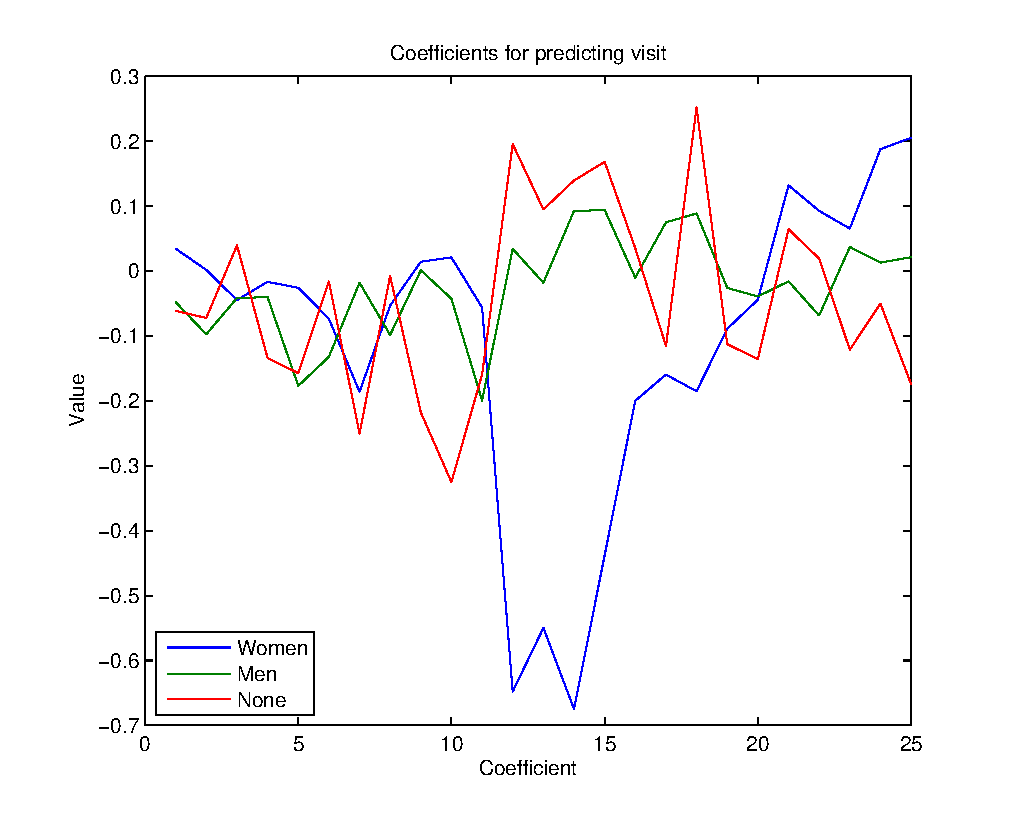
\includegraphics[width=5.7cm]{visitCoeff}  
 \end{minipage}
 \begin{minipage}{5.7 cm}
	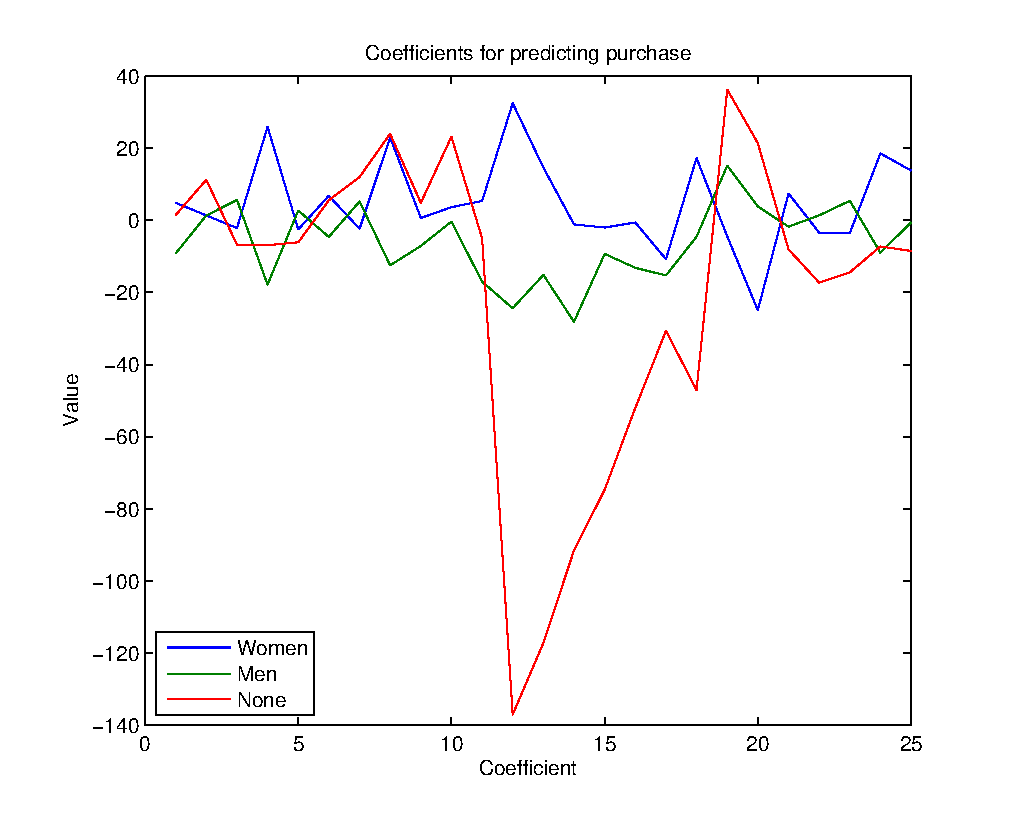
\includegraphics[width=5.7cm]{purchaseCoeff}  
 \end{minipage}
 \begin{minipage}{5.7 cm}
	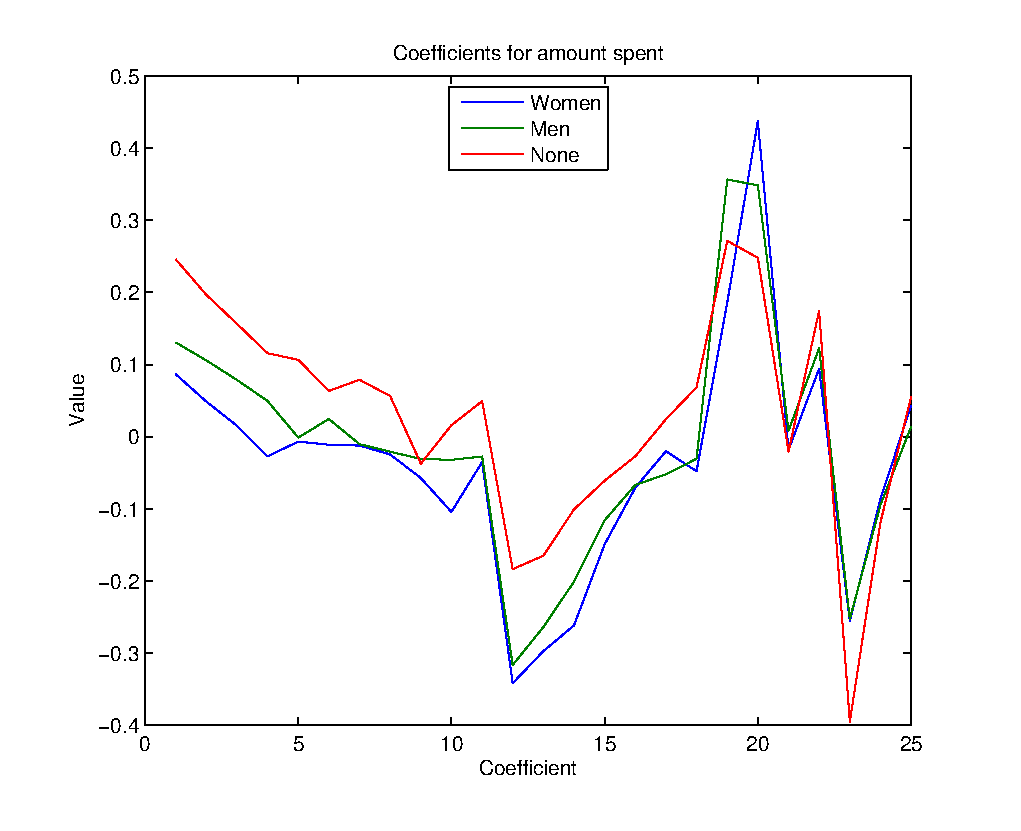
\includegraphics[width=5.7cm]{spendCoeff}  
 \end{minipage}
 \caption{The $\beta$-Coefficients for the three treatments for predicting visit, purchase and amount spend (from left to right)}
 \label{betacoeff}
\end{figure*}

\begin{figure}[htbp]
\begin{tabular}{|l|cc|cc|}
\hline
\multirow{2}{*}{Treatment}
 & \multicolumn{2}{|c|}{$E[\mbox{Spend}|\mbox{Trt}]$}
  & \multicolumn{2}{|c|}{RSSE} \\
\cline{2-5}
&       	mean &   std & 	mean &   std \\
\hline
Men   & 	1.4632 &0.0196 & 0.2275 &0.0115\\
Women & 	1.0887& 0.0449 & 0.1991& 0.0096\\
None 	&  0.6905& 0.0698 & 0.1578& 0.0275\\
\hline
\end{tabular}
\caption{E[Spend|Trt] means the expected amount that the test examples are predicted to spend per person. This is calculated 5 times, yielding a mean and standard deviation.  E[Spend|Trt]= 1/N * sum E[Spend|xi,Trt]. RSSE means the RSSE per example of the predicted-actual spend. $RSSE = 1/N * sqrt( sum (y_i - E[Spend|x_i,Trt])^2$}
\end{figure}

%Trivial Case
\begin{figure}[htbp]
\begin{tabular}{|l|cc|cc|}
\hline
\multirow{2}{*}{Treatment}
 & \multicolumn{2}{|c|}{$E[\mbox{Spend}|\mbox{Trt}]$}
  & \multicolumn{2}{|c|}{RSSE} \\
\cline{2-5}
&       	mean &   std & 	mean &   std \\
\hline
Men   & 	
    1.4226  &  0.0638   & 0.2686  &  0.0479 \\
Women & 	1.0772   & 0.0794  7  0.2279  &  0.0431\\
None 	&   0.6528  &  0.0306  &  0.1735 &   0.0418\\
\hline
\end{tabular}
\caption{The trivial results for the same testing as in Figure \ref{nontrivial}}
\label{trivial}
\end{figure}

%------------------------------------------------------------------------

\section{Conclusion}
The results show that e-mail  advertisement makes a difference. The men's email leads to a higher outcome of 0.77 USD, the women's mail to a higher outcome of 0.40 USD. That means, that no more than this amount should be invested to increase sales. Table \ref{salestable} shows the maximum amount one should spend for the Men's and Women's email campaigns to increase the sales for different numbers of customers. 

It is recommended to send advertisement emails to customers who have previously purchased merchandise, spent money recently and are in a history segment between \$ 100 and \$ 500 

Unfortunately it is very hard to predict the habitual buying behavior of single customers, since this behavior is very randomly distributed and depends on too many other influences. Using our simple models however, we can sometimes see which features that are important in regards to for example how much a person will spend given a treatment. The question of which campaign that has the greatest influence could have been answered with simple statistics. Machine learning only strengthens the confidence in the validity of this result and gives us an opportunity to see what factors were influential.

\begin{figure*}[htbp]
  \centering
 \begin{tabular}{|l|l|l|l|l|l|l|l|l|}
  \hline
   Number of
Customers & 500   & 1,000 & 2,500   & 5,000   & 10,000  & 20,000   & 50,000   & 100,000 \\
\hline
   USD for Men's mail  & 386,- & 773,- & 1,932,- & 3,864,- & 7,727,- & 15,454,- & 38,635,- & 77,270  \\
   USD for Women's mail  & 199,- & 398,- & 996,- & 1,991,- & 3,982,- & 7,964,- & 19,991,- & 39,820,- \\
  \hline
 \end{tabular}
\caption{Maximum amount one should spend for the Men's and Women's email campaigns to increase sales depending on the number of customers}
	\label{salestable}
\end{figure*}






\nocite{hillstrom08, bishop06,bottou11,elkan11}

{\small
\bibliographystyle{ieee}
\bibliography{egbib}
}

\end{document}
